\documentclass{article}
\usepackage{amssymb}
\usepackage{authblk}
\usepackage{color}
\usepackage{graphicx}
\usepackage[utf8]{inputenc}
\usepackage{natbib}
%\usepackage[style=authoryear,backend=biber]{biblatex}

% FIXME: This is for automatic sizing of nested parentheses
%\usepackage{nath}
%\delimgrowth=1

\usepackage{nth}
\usepackage{soul}

\begin{document}

\title{CSCI435 Project}
\author{Paul Foster
	\thanks{Email: \texttt{pf981@uowmail.edu.au}}
	\thanks{Student Number: \texttt{3648370}}}
\affil{University of Wollongong}
\date{2013 Spring}

\maketitle

\renewcommand\abstractname{Executive Summary}
\begin{abstract}
\hl{FIXME: TODO - do not use what it is currently}
Gwynville Airport Authority has requested evaluation of some computer vision
technologies that they plan to deploy as part of their security and surveillance system.
The system should be able to count the number of people in a waiting room area based
on the image captured by a camera suitably located to `see'' the faces of passengers. Furthermore the Authority would like to recognize a speci.c group of people that are known
to be frequent users. The idea is to update their `Frequent Users'' card whenever they
are recognized in the Airport premises. In this case they intend to use a face recognition
algorithm that can learn from a dataset comprising the faces of these citizens.
\end{abstract}

Definitions: face space

\section{Introduction}
Face detection and face recognition are two actively-researched and important topics in computer vision. Both of these tasks are performed frequently and easily by humans however no current automated system exists that can be deployed effectively in an unconstrained setting \cite{sinha2006face}.

Earlier forms of facial detection and recognition involved holistic methods such as Eigenfaces\cite{turk1991eigenfaces} and Fisherfaces\cite{belhumeur1997eigenfaces}. However, more recently, local descriptors such as Local Binary Patterns (LBP)\cite{ahonen2004face} and Local Intensity Distribution (LID)\cite{nguyen2011local} have gained attention due to their efficiency and tolerance to pose and illumination changes.
Face recognition technology has significantly progressed since the proposal of the Eigenface method in 1987. Given that most individuals can only identify a few thousand people, under constrained conditions (such as fixed facial expression and lighting) and a very large number of classifications, automated face recognition can perform better than human recognition \cite{li2011handbook}.

\hl{FIXME: History of FACE DETECTION}

There are numerous commercial and law-enforcement applications for face detection and recognition including advanced video surveillance, user authentication and suspect tracking \cite{zhao2003face}. The effectiveness of these applications rely on the efficiency and accuracy of the underlying algorithms. In this report, we will compare the efficiency and accuracy of 4 facial recognition algorithms: Eigenfaces, Fisherfaces, Local Binary Patterns (LBP) and Local Intensity Distributions (LID). We will also investigate the efficiency and performance of Haar feature-based cascade classification for face detection and discuss how these algorithms can be applied by the Gwynville Airport Authority for their security and surveillance system.


\section{Data Preparation}
The individual face data given consisted of between 9 and 14 photos each of the faces of 11 students. The images were converted to grayscale then were scaled down and cropped to 128*128. This was achieved by uniformly scaling the image such that the smaller dimension was equal to 128 pixels. The 128*128 rectangle centred at the centre of the image was then used as the cropped image. 128*128 was chosen because it was large enough to provide good results but not so large as to be computationally problematic.

For group photos, where we wanted to use the face-counting algorithm, the photo was uniformly scaled such that its area was approximately 640*480 to reduce computation.

\subsection{Training/Testing Split}
For cross validation, the student photos were split into two sets: a training set and a validation set. They were used to train the classification model and measure the performance of the model respectively. There can be no overlap in these two sets as trained images will obviously be classified correctly and will not give accurate real-world performance measures.

The proportion of the size of the training set to the size of the validation set was chosen to be \hl{FIXME:SOMETHING, look at cross validation - involves mutiple sampling. Also, maybe put this splitting into the algorithm results section as it doesn't apply to Haar}. The choice of this ratio is a balance between better classification with more training data, or more accurate performance estimates with more test data.

\hl{some\%} of the data were used to train the model and the other \hl{some\%} were used to test its performance.

\section{People Counting Algorithms}
Data Prep

\subsection{Haar}
Technical description
\subsubsection{Parameter Optimisation}
There were four parameters to consider with the Haar classifier: double scaleFactor, int minNeighbors, Size minSize and Size maxSize.

I found that more faces were detected (either correctly or as false positives) as scaleFactor was increased and minNeighbors was decreased.

Starting at minNeighbors=3, I incrementally increased its value until a sufficient amount of noise (false positives) was removed. I chose the value that was the largest that still detected every face in the image. This value was 9.

Similarly for scaleFactor, I started at 1.01 and increased its value until every face was detected and there were no false positives. I found this value to be 1.017. 

I used opencv's pre-trained xml file.

I chose to leave minSize and maxSize unspecified as this would allow for detection of people at significantly varying distances to the camera.
scaleFactor=0.017; minNeighbors=9

\begin{figure}
\centering
%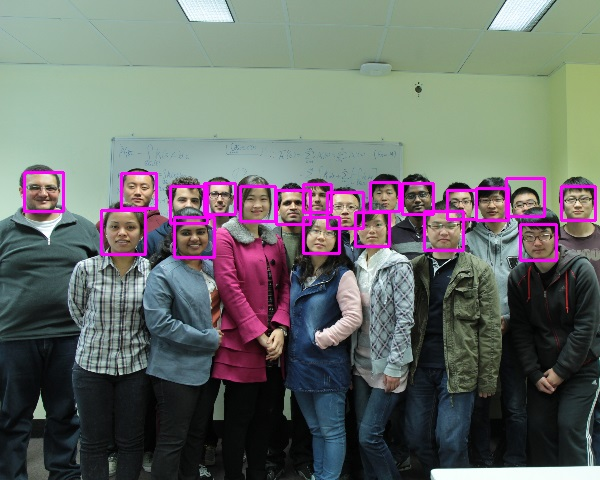
\includegraphics[width=0.7\linewidth,natwidth=10,natheight=10]{waiting_room_detected.jpg}
%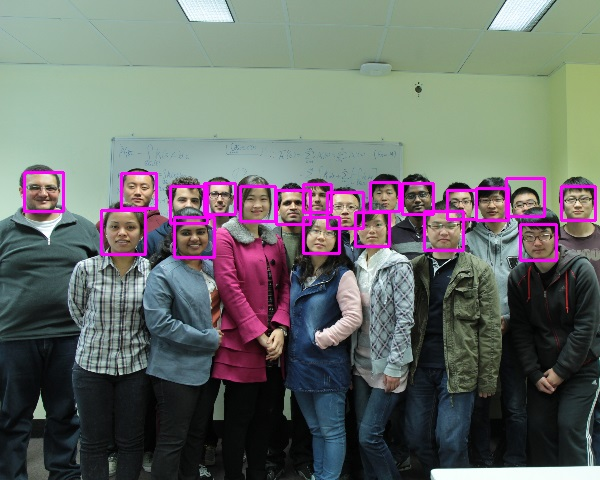
\includegraphics[width=0.1\linewidth]{waiting_room_detected.jpg} % FIXME: If this is too big it ends up restarting the page numbering
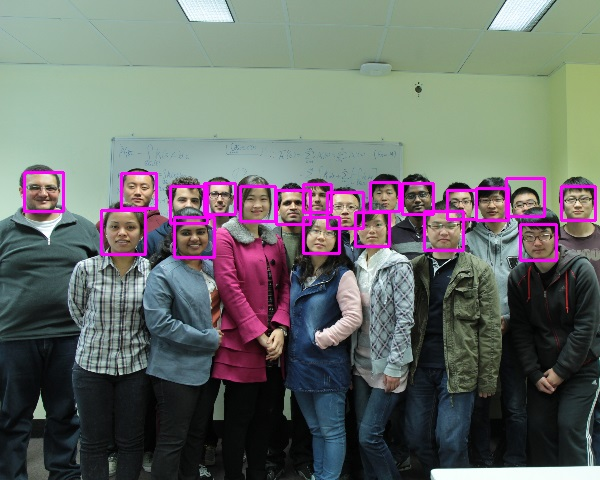
\includegraphics[scale=1]{waiting_room_detected.jpg}
%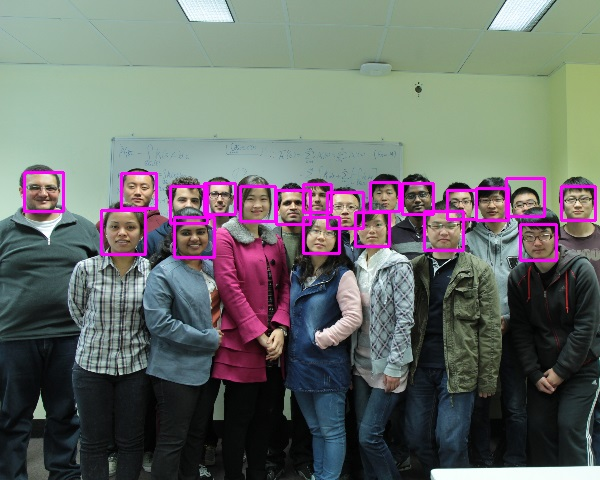
\includegraphics[width=250px,height=250px]{waiting_room_detected.jpg}
\caption{Haar Cascade Classifier FIXME: If this is big it resets page num for some reason; FIXME: REDO - YOU HAVE CROPPED SOMEONE OUT!!!}
\label{fig:haar_cascade}
\end{figure}


%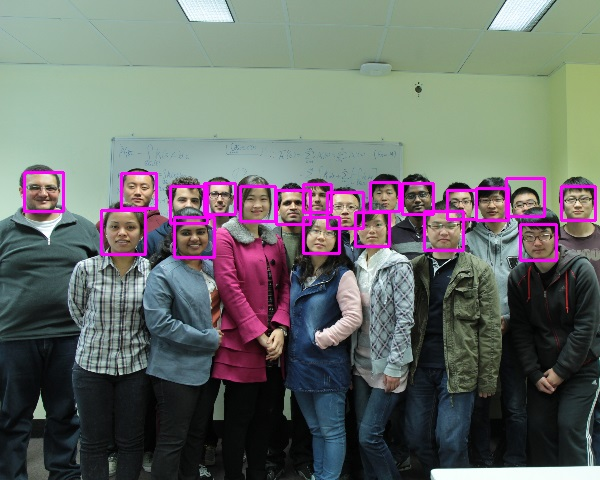
\includegraphics[width=0.7\linewidth]{waiting_room_detected.jpg}
%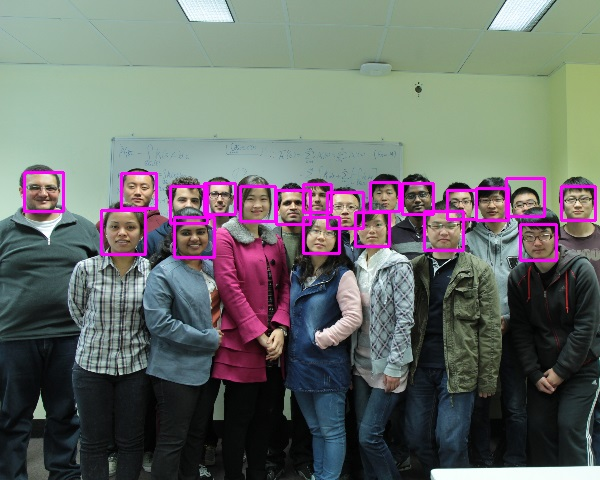
\includegraphics{waiting_room_detected.jpg} % FIXME: Too big
%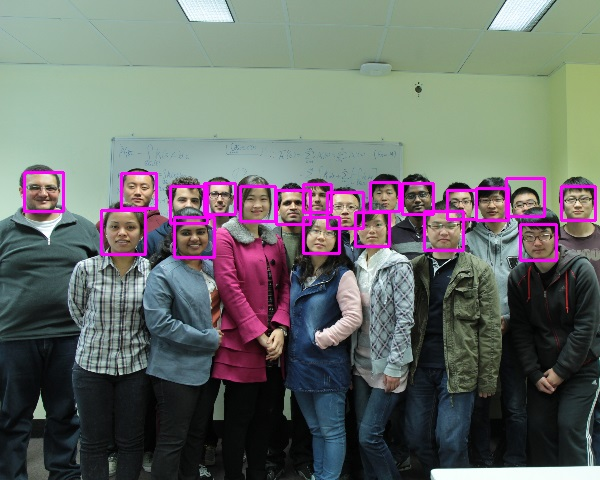
\includegraphics[scale=1]{waiting_room_detected.jpg} 

\subsection{Local Binary Patterns}
Technical description
\subsubsection{Parameter Optimisation}
Data Prep

\subsection{Comparison}
Advantages and disadvantages of each algorithm with side-by-side images after parameter optimisation


\section{Face Recognition Algorithms}
Data Prep

\subsection{Eigen Face}
If we describe the collection of all images of the face of an individual as a vector space, then we can describe every such image through a linear combination of the spanning vectors of that space.

The goal is to find the principal components of the training data, called eigenfaces. These eigenfaces form a basis for every image of this person’s face. That is, every image of this person’s face can be described as a linear combination of the eigenfaces. Furthermore, every image of this person’s face can be approximated by a linear combination of the eigenfaces with the largest eigenvalues.

The Eigenfaces are computed in the following way. Given $M$ training images with dimensions $h$*$w$, we consider each image as an $D$-dimensional vector where $D = hw$.

\vspace{12pt} \noindent Let $S$ be the set of the $M$ training images.
\begin{equation}
	S = \left\{\Gamma_1, \Gamma_2, \Gamma_3, \ldots, \Gamma_M\right\}
\end{equation}
Let $\Psi$ denote the average face of $S$. That is,
\begin{equation}
	\Psi = \frac{1}{M}\cdot\sum_{n=1}^{M}\Gamma_n
\end{equation}
Let $\Phi_i$ denote the difference between the $i$\textsuperscript{th} training face and the average.
\begin{equation}
	\Phi_i = \Gamma_i - \Psi
\end{equation}
Constructing the covariance matrix, $C \in \mathbb{R}^{D\times D}$, we get
\begin{equation}
	C = \frac{1}{M}\cdot\sum_{n=1}^{M}\Phi_n \Phi_n^T
	  = AA^T
\end{equation}
Where $A = [\Phi_1 \Phi_2 \ldots \Phi_M]$

We wish to calculate the eigenvectors of $C$. However, this is typically a computationally infeasible task.

We construct $L \in \mathbb{R}^{M\times M}$ as $L = A^T A$ such that $L_{mn} = \Phi^T_m \Phi_n$

\subsubsection{Parameter Optimisation}
Data Prep

\subsection{Fisher Face}
The main advantage of this method is that it is invariant to different light sources. Extensive experimental results show that Fisherface has lower error rates than eigenface on the havard and yale face detection databases. (See the abstract of the pdf).

Although this method has advantages when subject to different lighting conditions, this advantage is not really applicable to our purposes as the camera will likely be uniformly lit. (Maybe it will be important if it is sometimes lit by natural light and sometimes lit by artificial light depending on the time of day.


Technical description
\subsubsection{Parameter Optimisation}
Data Prep

\subsection{Local Binary Patterns}
The LBP descriptor describes a pixel as an $P$-bit binary number based on the values of $P$ points on the circumference of a circle of radius $R$ centred at the pixel. This number becomes its label.
Because LBP converts pixels to an binary number, computations can be done with integer arithmetic which results in significant performance advantages over the other methods which use floating-point arithmetic.

We will define a uniform pattern to be a binary pattern containing at most two bitwise transitions from 0 to 1 or 1 to 0. \cite{ojala2002multiresolution}

Let $(P, R)$ denote the pixel neighbourhood of $P$ evenly-spaced points on the circumference of a circle of radius $R$.

Let $LBP^{u^2}_{P,R}\cdot$ denote the LBP operator in a $(P, R)$ neighborhood using only uniform patterns ($u^2$).

$n$ neighboring pixels 

The image is equally split into $X$ columns and $Y$ rows. Each of these regions is given a weight.
\subsubsection{Training}
Each of the training images trained in the following way. The LBP for the pixels inside each region is calculated.
\hl{Something to do with a histogram...
Each regions pixel classifications are put into a histogram. This histogram represents the pattern of that region.
Oh, and then you do the bag of words thing that we did with assig2. But how do we combine all the training images of one person into one thing to compare against? This is the same problem as we are having with LID. IDEA: You could have each image "vote" whether they are similar. The class with the most votes wins. You would have to take into account the fact that there are different numbers of training data}

\subsubsection{Parameter Optimisation}
Data Prepsssss

\subsection{Local Intensity Distribution}
\hl{LID does 2 things: uses a computationally efficient distance measure for kmeans clustering, Defines a LID descriptor, other stuff. Insert diagram to illustrate what neighboring pixels are in LID. Do the same for LBP.

You could use SI}

Local Intensity Distribution (LID) descriptors can be used to describe the features of an intensity image by capturing the distribution of local intensity differences. Similarly to LBP descriptors, LID descriptors are insensitive to illumination changes.

Let $I(x,y) : \mathbb{Z}^2 \rightarrow \mathbb{R}$ denote the intensity image of an image with $N$ pixels and let $p = (x,y) \in \mathbb{Z}^2$ be an arbitrary point in the domain of $I$. We define $LID_{N,R}(p) : \mathbb{Z}^2 \rightarrow \mathbb{R}^N$ as
\begin{equation}
   % \label{simple_equation}
   LID_{N,R}(p) = \langle d(p_1,p), \ldots, d(p_n,p)\rangle
\end{equation}
where $d(p_i,p) = I(p_i) - I(p)$ and $p_i = (x_i, y_i) \in \mathbb{Z}$ is such that $max\{|x_i - x|, |y_i - y|\} = R$. % FIXME: There must be a better way to describe this rectangle (perimeter) than using this max.

We can determine the dissimilarity $D(I_1, I_2)$ between two images through the Kullback-Leibler (KL) distance \cite{kullback1951information}.
\begin{equation}
   % \label{simple_equation}
	D(I_1, I_2) = \frac{KL\left(p_{I_1}(v) \| p_{I_2}(v)\right) +
	              KL\left(p_{I_2}(v) \| p_{I_1}(v)\right)}{2}
\end{equation}
\hl{FIXME: Do some handwaving, then}
\begin{equation}
   % \label{simple_equation}
	KL(p_1(v) \| p_2(v)) = \sum_{i=1}^{N}KL(p_1(v_i) \| p_2(v_i))
\end{equation}

\subsubsection{Parameter Optimisation}
Data Prep

\subsection{Comparison}
Advantages and disadvantages of each algorithm with side-by-side images after parameter optimisation


\section{Recommendation}
conc

When implementing the airline actual thingo, you should constantly add to your training data.
So when you see a person and you confidently classify them as known, add that image to the training data.
If you see the same unknown face, calculate its characteristics and make it known. This is what they want because then they would be able to tell who is frequent without having to manually train.
The implementation you are looking for would be to use the face counter and then send each face into the second algorithm which will attempt to identify them.
It is critical that the camera have a frontal face view as the training data for the Haar cascade classifier was frontal faces.


\section{Conclusion}
Write your conclusion here. \citep{guyon1997scaling} \citep{belhumeur1997eigenfaces}
\hl{bias-variance dilemma; Maybe use ROC curve to evaluate performance (IS THIS EVEN APPLICABLE?)

Will not detect clipped faces or faces rotated.

All these faces were trained with the same illumination and facial hair etc on the same day. It will likely not perform well on images of different illumination.

We found that eigen and fisher took significantly longer to train and compute
}

\nocite{*} % List uncited references % FIXME: Doesn't work
\bibliographystyle{plain}
\bibliography{references}

\end{document}
% FIXME: There is a problem: The page numbers restart in the middle :-( Don't know why
% FIXME: For training, we don't really test false positives. We could give it some faces not in the dataset.
% FIXME: Look at http://people.wku.edu/qi.li/teaching/595_BA/ba16_Eigenface.pdf for cross-validation in determining the best split